\documentclass{article}
\usepackage[T1]{fontenc}
\usepackage{lmodern}
\usepackage{graphicx}
\usepackage{amsmath,amssymb}
\usepackage[a4paper,margin=2cm]{geometry}
\usepackage[absolute,overlay]{textpos}
\setlength{\TPHorizModule}{1mm}
\setlength{\TPVertModule}{1mm}
\usepackage[indonesian]{babel}
\usepackage{hyperref}
\setlength{\emergencystretch}{2em}
% unit: Halaman 33

\begin{document}

% === Halaman 33 (llm) ===

\vspace{106.92mm}

\section*{Kelemahan Mode CBC}

\vspace{106.92mm}

\begin{enumerate}
    \item Kesalahan satu bit pada sebuah blok plainteks akan menghasilkan kesalahan pada blok cipherteks yang berkoresponden dan kesalahan tersebut merambat ke semua blok cipherteks berikutnya.
    \vspace{50mm}
    \item Tetapi, hal ini berkebalikan pada proses dekripsi. Kesalahan satu bit pada blok cipherteks hanya mempengaruhi blok plainteks yang berkoresponden dan satu bit pada blok plainteks berikutnya (pada posisi bit yang berkoresponden pula).
\end{enumerate}

% deskripsi: Diagram proses enkripsi pada mode CBC (Cipher Block Chaining) yang menunjukkan aliran data dari plainteks P ke cipherteks C menggunakan kunci K dan Initialization Vector (IV).
% bbox normalisasi: [0.5300, 0.1200, 0.9800, 0.4800]
\begin{textblock*}{94.50mm}(111.30mm,35.64mm)
\noindent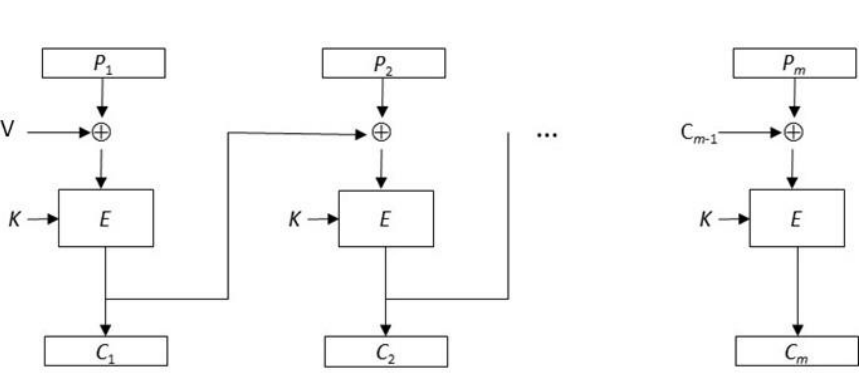
\includegraphics[width=94.50mm,height=106.92mm]{../../images/llm/page_033_img_01.png}%
\end{textblock*}

% deskripsi: Diagram proses dekripsi pada mode CBC (Cipher Block Chaining) yang menunjukkan aliran data dari cipherteks C kembali menjadi plainteks P menggunakan kunci K dan Initialization Vector (IV).
% bbox normalisasi: [0.5300, 0.5300, 0.9800, 0.8900]
\begin{textblock*}{94.50mm}(111.30mm,157.41mm)
\noindent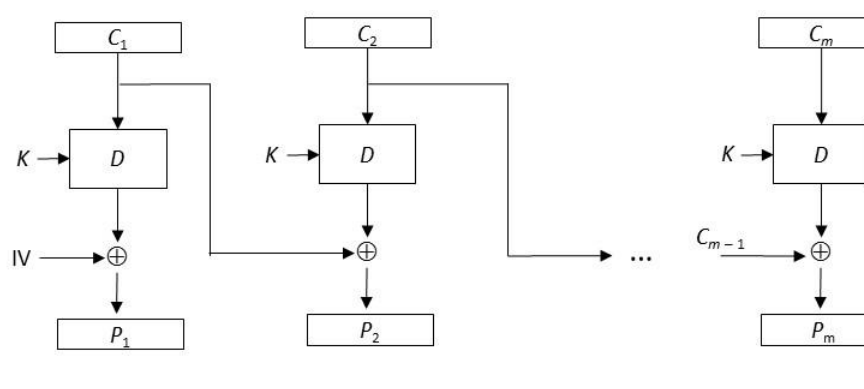
\includegraphics[width=94.50mm,height=106.92mm]{../../images/llm/page_033_img_02.png}%
\end{textblock*}

\end{document}
